% !TeX program = xelatex
\documentclass[UTF8,fontset=fandol,a4paper,11pt]{ctexart}
\usepackage[margin=25mm]{geometry}
\usepackage{amsmath,amssymb,amsthm,graphicx,booktabs,array,tabularx,subcaption}
\usepackage[hidelinks]{hyperref}
\graphicspath{{figures/}}
\usepackage[backend=biber,style=numeric,sorting=none]{biblatex}
\addbibresource{references.bib}
\title{室内温度校正：排版练习}
\author{研究助理}
\date{}
\begin{document}
\maketitle
\begin{abstract}本文使用六条教学合成观测比较两种温度校正结果，演示论文结构、图表与文献的组织。本文不报告真实科研发现。\end{abstract}
% !TeX root = ../main.tex
\section{引言}\label{sec:intro}
本项目比较两种室内温度校正方案。所有数据均为教学合成数据，
只用于练习论文排版，不能据此声称算法具有实际科研效果。
\emph{可复现的排版}要求正文、数据与引用能够一起交付。
数据版本为 \texttt{sensor\_v2}，抽查比例为 20\%。
\footnote{本实验不收集真实受试者数据。}
方法见第~\ref{sec:method} 节，结果与局限见第~\ref{sec:results} 节。
\subsection{研究问题}
比较 Baseline 和 Calibrated 在六个时刻的误差。
\begin{itemize}
  \item 保留原始观测；
  \item 图、表和正文使用同一组数据。
\end{itemize}
\begin{enumerate}
  \item 读取数据；\item 计算误差；\item 复核结果。
\end{enumerate}
\begin{description}
  \item[真实值] 本教学数据中给定的参照温度。
  \item[预测值] 两种方法给出的温度。
\end{description}

% !TeX root = ../main.tex
\section{方法}\label{sec:method}
令 $y_i$ 为真实值，$\hat y_i$ 为预测值，样本数 $n=6$。
采用式~\eqref{eq:rmse} 的均方根误差，单位与温度相同。
\begin{equation}
 \operatorname{RMSE}=\sqrt{\frac{1}{n}\sum_{i=1}^{n}(\hat y_i-y_i)^2}.
 \label{eq:rmse}
\end{equation}
\begin{align}
 e_i &= \hat y_i-y_i,\label{eq:error}\\
 \operatorname{MSE} &= \frac{1}{n}\sum_{i=1}^{n}e_i^2.\label{eq:mse}
\end{align}
平均绝对误差为 $\operatorname{MAE}=\frac{1}{n}\sum_{i=1}^{n}|e_i|$，
它与 RMSE 一般不同；本组样本中两者恰好相等。
用分段函数标记是否超过容差：
\begin{equation*}
 q_i=\begin{cases}1,&|e_i|\leq 0.5,\\0,&|e_i|>0.5.\end{cases}
\end{equation*}
两个误差样本组成列向量 $\boldsymbol e=\begin{pmatrix}e_1\\e_2\end{pmatrix}$。

% !TeX root = ../main.tex
\section{结果与局限}\label{sec:results}
图~\ref{fig:comparison} 的子图~\ref{fig:baseline} 和~\ref{fig:calibrated}
分别展示两种方法；表~\ref{tab:metrics} 给出汇总。
Calibrated 的 RMSE 为 $0.500\,{}^\circ\mathrm{C}$，
比 Baseline 的 $1.000\,{}^\circ\mathrm{C}$ 低 50\%。
这一比较仅对当前六条合成样本成立，不代表真实环境中的泛化效果。
\begin{figure}[htbp]
 \centering
 \begin{subfigure}{0.48\linewidth}
  \centering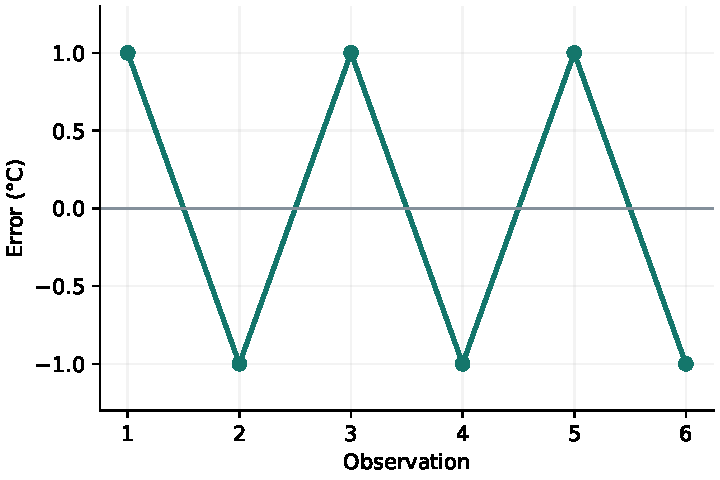
\includegraphics[width=\linewidth]{baseline.pdf}
  \caption{Baseline}\label{fig:baseline}
 \end{subfigure}\hfill
 \begin{subfigure}{0.48\linewidth}
  \centering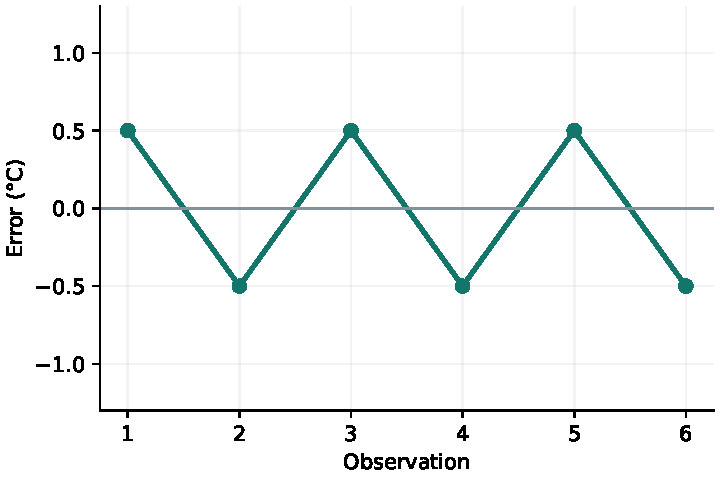
\includegraphics[width=\linewidth]{calibrated.pdf}
  \caption{Calibrated}\label{fig:calibrated}
 \end{subfigure}
 \caption{两种方法的误差对比（教学合成数据）。}\label{fig:comparison}
\end{figure}
\begin{table}[htbp]
 \centering
 \caption{温度误差汇总（教学合成数据）。}\label{tab:metrics}
 \begin{tabular}{lrr}
  \toprule
  \multicolumn{1}{c}{方法} & \multicolumn{2}{c}{误差（$^\circ$C）}\\
  \cmidrule(lr){2-3}
   & RMSE & MAE\\
  \midrule
  Baseline & 1.000 & 1.000\\
  Calibrated & 0.500 & 0.500\\
  \bottomrule
 \end{tabular}
\end{table}

\section{排版资料}
文档组织参考\cite{lamport1994}，排版背景参考\cite{knuth1984}。
文献\cite{einstein1905}仅作期刊条目格式示例，不作为本方法依据。
\printbibliography[title={参考文献}]

\end{document}
